\chapter{Simulator software}

In this chapter, I present the simulator software I wrote. I discuss the currently available solutions, why I chose to write the software, the architecture, the components and design patterns I used, the challenges I faced during the development and the solutions I found.

\section{Currently available solutions}

Since publicly accessible quantum computers currently only have around 5-10 qubits, it is not viable at the moment to run quantum walks on a real quantum computer. Hence why, when I started researching quantum walks, I quickly began looking into simulator software. While there are many of these currently available (for example \cite{Portugal} contains an extensive selection of open-source simulator software), most of them have at least one of the following issues:

\begin{enumerate}
\item Not maintained and developed anymore: the last commit was years ago.
\item Written in a low-level language, like C++, in a script-like fashion, with a prominent focus on memory and performance optimization while neglecting readability, modularity and extensibility.
\item Works exclusively on a specific type of graph, for example, n-dimensional lattices only.
\item Unable to compare and contrast classical and quantum walks on the same graph, running only quantum simulations.
\item Hard to understand as a novice.
\end{enumerate}

There is no general, open-source solution available that is designed and developed using sound software engineering practices and an architecture that allows for experimentation with different kinds of graphs with both classical and quantum simulations available.

I intend my solution to be valuable for research purposes while also providing a readable open-source codebase for college students to study the algorithm.

\section{Architecture}

The architecture of my simulator program employs the Strategy design pattern, which is described in the following way:

''Define a family of algorithms, encapsulate each one, and make them interchangeable. Strategy lets the algorithm vary independently from clients that use it.''~\cite{DesignPatterns}

\begin{figure}[H]
  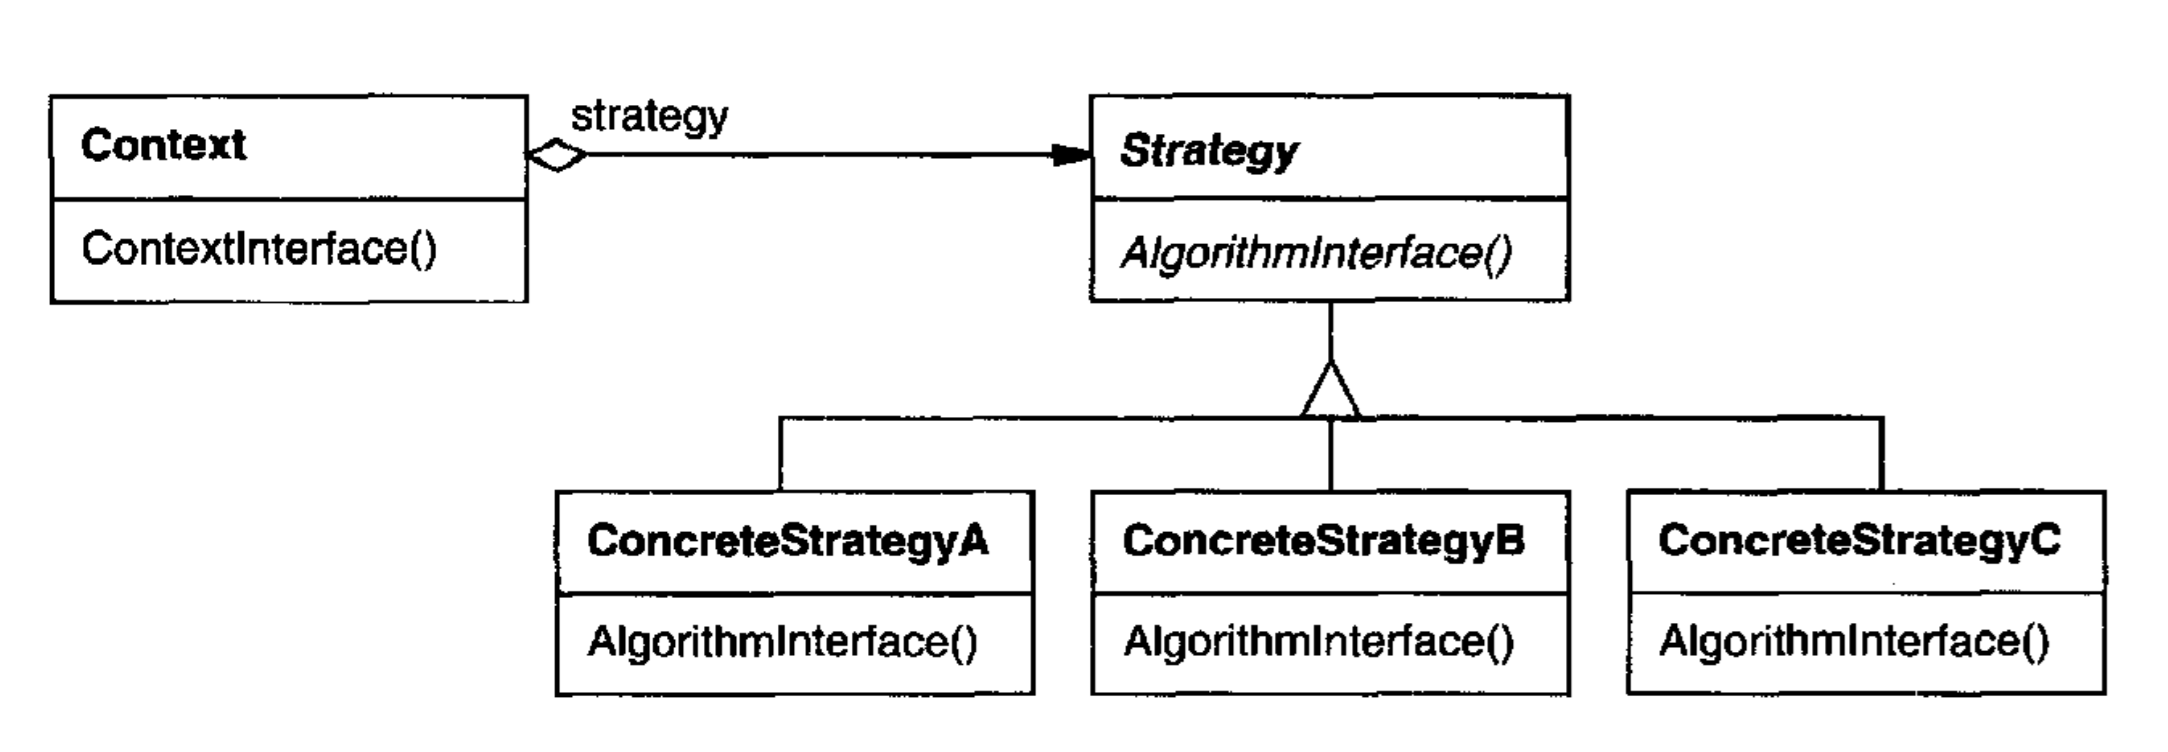
\includegraphics[width=\linewidth]{./figures/program/strategy.png}
  \caption{UML diagram for the Strategy design pattern from~\cite{DesignPatterns}}
\end{figure}

This is a great design pattern for research purposes since it facilitates experimentation with various algorithms for the same purpose. It also makes the code easily readable, as the Strategy interface provides an abstraction layer between the Context and the concrete implementation.

\section{Language choice}

With the specified goals and the architecture in mind, I needed a language that is object-oriented, easily readable by beginners and has extensive capabilities for using complex numbers, linear algebra and plotting. For these purposes, I choose the Python language. Python is concise, it reads like pseudocode and has libraries such as NumPy, SciPy and Matplotlib, and so on, covering all areas of data science. Furthermore, it is well-known and extensively used by researchers with no software engineering background, allowing for easier collaboration.

\section{High level design}

The source code of the software can be divided into three parts:

\begin{itemize}
    \item Graph models
    \item Simulators
    \item Running, configuration and result collection
\end{itemize}





\section{Gráfmodellek}

A félév során sokféle gráfon futtattam szimulációs kísérleteket, melyek során több problémába ütköztem. Kezdetben úgy oldottam meg a szimulációkat, hogy a célgráfok szomszédossági mátrixait generáltam le, egyben a memóriában tartva azokat és a lépések során a megfelelő csúcshoz tartozó sorokat lekérdezve.

Ezzel a módszerrel több probléma is jelentkezett. Az első gondot az okozta, hogy a szomszédossági mátrix mérete a csúcsszám négyzetével arányos, ezért pár ezer csúcsú gráfot már nem tudtam a memóriában tartva szimulálni. A második probléma pedig az volt, hogy a szomszédossági mátrixos ábrázolás nagyon távol esett az emberi szempontból természetes ábrázolástól. A kvantumbolyongásos szimulációkat tipikusan nem véletlenszerű gráfokon szokták kipróbálni, hanem jól ismert struktúrával rendelkező gráfokon. Ilyen gráfok például a ,,súlyzók''
vagy a ragasztott bináris fák.

A súlyzó gráf két egyforma méretű kört tartalmaz, mindkét körből kiválasztva $k - k$ darab csúcsot, melyek teljes páros gráfot alkotnak (a súlyzó középső rúdját). A körökben pedig nem csak az egymás melletti csúcsok között fut él, hanem futhat él minden $i.$ csúcs között is. A ragasztott bináris fában két egyforma méretű teljes bináris fa leveleit szembefordítjuk és a két oldali levelek közé egy teljes páros gráfot készítünk.

A fenti leírásból látható, hogy az ember számára természetes leírás a gráfokat ismert részgráfok kompozitjaként adja meg. A félév során olyan architektúrát alakítottam ki a szimulációkhoz, mely ezt a szemléletet támogatja. A szomszédossági mátrixos tárolási mód helyett pedig a szomszédossági orákulum megközelítést használva nagyban csökkent az alkalmazás memóriaigénye. Ennek a megközelítésnek a lényege, hogy az ismert struktúrájú gráfokra nem tárolok a memóriában szomszédossági információt, helyette biztosítok egy függvényt, amely a bemeneti paraméterként kapott csúcsindexre kiszámolja a vele szomszédos csúcsok indexeit.

A félév során a következő nevesített részgráfok szomszédossági orákulumját implementáltam:

\begin{itemize}
  \item BinaryTree
  \item Bipartite
  \item Circle
  \item Path
  \item Random
\end{itemize}

\change{Új: Hiperkocka}

\begin{center}
  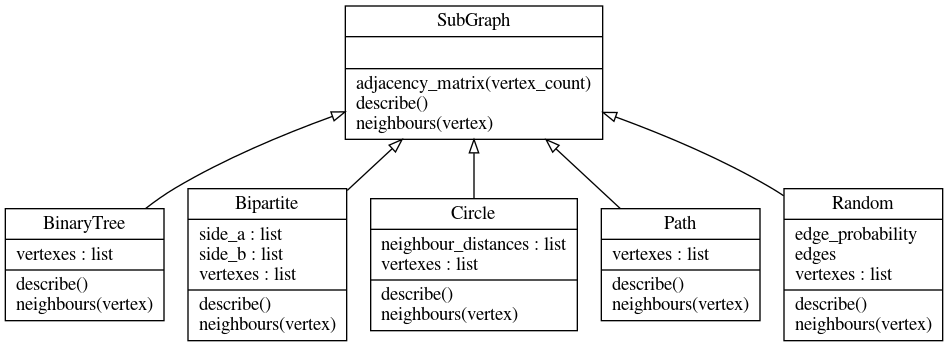
\includegraphics[width=\linewidth]{./figures/program/subgraph.png}
\end{center}

Ezen részgráfokból épülnek fel az alábbi kompozit gráfok:
\begin{itemize}
  \item Dumbbell
  \item GluedBinary
\end{itemize}

\begin{center}
  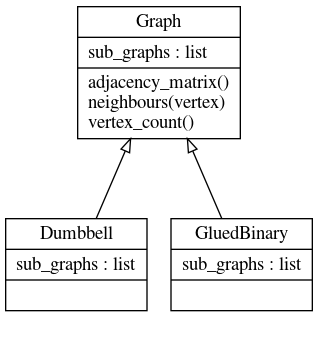
\includegraphics[width=0.4\linewidth]{./figures/program/graph.png}
\end{center}

\section{Szimulátorok}

A szimulátor osztályok közül a klasszikus tetszőleges kompozit gráfot tud
fogadni.

\change{Itt fontos átírni, hogy a kvantumszimulátor mostmár d-regulárist is tud!}

A kvantumszimulátor jelenleg a kvantumbolyongás egy speciális esetét, az egyenesen való bolyongást képes kezelni, mely a 2-regularitása miatt egyszerűbben implementálható. Hosszú távú cél a k-reguláris, illetve az általános gráfokra kiterjeszteni ezt a szimulátort.

\begin{center}
  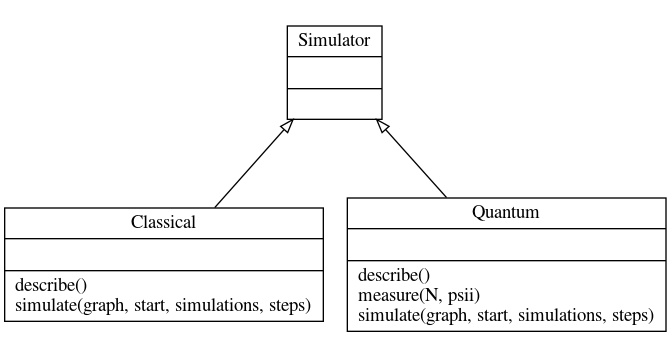
\includegraphics[width=0.8\linewidth]{./figures/program/simulator.png}
\end{center}

\section{Futtatás, konfiguráció, eredmények ábragenerátora}

\change{Itt van pár újdonság, pl. sajátértékek kiírása, stb.}

A fenti osztályok segítségével egy olyan keretrendszert alakítottam ki, melyben
nagyon gyorsan fel lehet 1-1 futtatást konfigurálni. A futtatás eredményeit egy
összesített Latex dokumentumba gyűjti a program. Ez tartalmazza a beadott gráf
részgráfjainak nevesített típusát, szomszédossági mátrixait, illetve a teljes
gráf szomszédossági mátrixát, valamint a szimulációk eloszlási eredményeit. A
következő fejezetben több ilyen ábrát is bemutatok.



Az első fázisban a szomszédossági mátrixot generáltam le teljesen. Ez nagyon sok memóriát használt, az unitér mátrix meg mégtöbbet, nagyon rosszul skálázódott. Lecseréltem spare mátrixokra, az már egy fokkal jobb.

\change{Mérés összehasonlítás: Mátrix, Spare mátrix, Orákulum grafikon.}

Ezután kipróbáltam a spare mátrixokat, de azok is picit sokak voltak, ugyan a gráfban sok a 0, de azért
így is nagyon skálázódott.

A legjobb megoldás az úgynevezett gráf orákulum volt. A gráf orákulum lényege, hogy nem tároljuk a szomszédossági mátrixot, helyette biztosítunk egy függvényt, mely on-the-fly a gráf adott csúcsindexét odaadva neki visszaadja hogy annak mik a szomszédai. A coin kis méretű, azt lehet tárolni (max fokszám * max fokszám), ezért azzal nem bajlódtam, bár éppen lehetne.